% Original TikZ artwork; source correspondence is in index.json.
% Requires tikz only; no additional library or shared style file.
\begingroup%
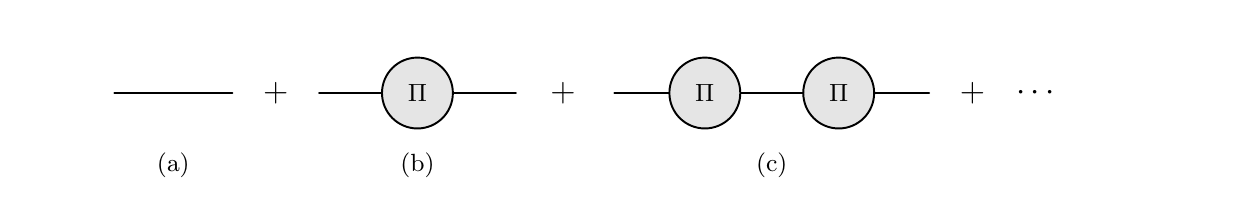
\begin{tikzpicture}[x=1cm,y=1cm,line width=0.7pt,line cap=round,line join=round]
\path[use as bounding box] (-7.6,-1.180) rectangle (7.6,0.830);
% Source occurrence S14-G02-01; original coordinate embedding.
\begin{scope}[shift={(-5.7500,0.0000)}]
\coordinate (g2a-in) at (-0.7500,0.0000);
\coordinate (g2a-out) at (0.7500,0.0000);
% Edge e1: in--out; path orientation in to out.
\draw (g2a-in) -- (g2a-out);
% Node in: fixed_external_endpoint.
% Node out: fixed_external_endpoint.
\end{scope}
\node[font=\large] at (-4.4500,0.0000) {$+$};
% Source occurrence S14-G02-02; original coordinate embedding.
\begin{scope}[shift={(-2.6500,0.0000)}]
\coordinate (g2b-in) at (-1.2500,0.0000);
\coordinate (g2b-out) at (1.2500,0.0000);
\coordinate (g2b-p1) at (0.0000,0.0000);
% Edge e1: in--p1; path orientation in to p1.
\draw (g2b-in) -- (g2b-p1);
% Edge e2: p1--out; path orientation p1 to out.
\draw (g2b-p1) -- (g2b-out);
% Node in: fixed_external_endpoint.
% Node out: fixed_external_endpoint.
% Node p1: effective_1PI_two_point_kernel.
\node[draw,fill=black!10,circle,minimum size=9mm,inner sep=0pt,font=\small] at (g2b-p1) {$\Pi$};
\end{scope}
\node[font=\large] at (-0.8000,0.0000) {$+$};
% Source occurrence S14-G02-03; original coordinate embedding.
\begin{scope}[shift={(1.8500,0.0000)}]
\coordinate (g2c-in) at (-2.0000,0.0000);
\coordinate (g2c-out) at (2.0000,0.0000);
\coordinate (g2c-p1) at (-0.8500,0.0000);
\coordinate (g2c-p2) at (0.8500,0.0000);
% Edge e1: in--p1; path orientation in to p1.
\draw (g2c-in) -- (g2c-p1);
% Edge e2: p1--p2; path orientation p1 to p2.
\draw (g2c-p1) -- (g2c-p2);
% Edge e3: p2--out; path orientation p2 to out.
\draw (g2c-p2) -- (g2c-out);
% Node in: fixed_external_endpoint.
% Node out: fixed_external_endpoint.
% Node p1: effective_1PI_two_point_kernel.
\node[draw,fill=black!10,circle,minimum size=9mm,inner sep=0pt,font=\small] at (g2c-p1) {$\Pi$};
% Node p2: effective_1PI_two_point_kernel.
\node[draw,fill=black!10,circle,minimum size=9mm,inner sep=0pt,font=\small] at (g2c-p2) {$\Pi$};
\end{scope}
\node[font=\large] at (4.4000,0.0000) {$+$};\node[font=\large] at (5.2,0) {$\cdots$};
\node[font=\small] at (-5.7500,-0.9200) {(a)};
\node[font=\small] at (-2.6500,-0.9200) {(b)};
\node[font=\small] at (1.8500,-0.9200) {(c)};
\end{tikzpicture}%
\endgroup%
